
% ------------------------------------------------------------------------
% Graph Grammar Documentation
% ===========================
%
\documentclass{article}
\usepackage{graphicx}
\usepackage{fancybox}
\usepackage{vmargin}
\title{ \huge{LSPExample} \\[4mm]
\small{ Graph grammar documentation generated by \textbf{AToM$^{3}$Doc} } }
%\author{ \small{Author: Denis Dube}} % <-- Put your name here
% Make decent margins
\setmarginsrb{1.5cm}{0.5cm}{1cm}{2.5cm}{12pt}{25pt}{12pt}{30pt}
% ------------------------------------------------------------------------
% Document Starts here:
% ------------------------------------------------------------------------
\begin{document}   
\maketitle         
\section*{  Rule \ref{fig:AddRoles} (Order 1): AddRoles}

\begin{figure*}[ht]
  \begin{center}
  \Ovalbox{
   \begin{tabular}{ c c c  }
    LHS &  $\rightarrow$& RHS \\
    \Ovalbox{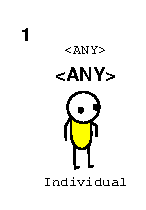
\includegraphics[width=0.1435\hsize]{Rule_1_LHS.eps}} & \
    $\rightarrow$&  \
    \Ovalbox{ 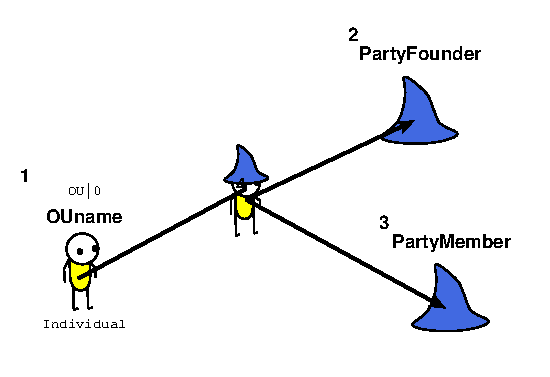
\includegraphics[width=0.6765\hsize]{Rule_1_RHS.eps}} \\
   \end{tabular}}
  \caption{AddRoles}
  \label{fig:AddRoles}
\end{center}
%\vspace{8pt}
\end{figure*}
%\hrule \vspace{6pt}
